\section{Presentation and Discussion of Results}
% =============================================================

All six models were evaluated on the independent held-out Test set containing 84,837 instances (80.3\% benign, 19.7\% anomalous). To perform a robust evaluation, we analyze model performance from three perspectives: the original imbalanced distribution, a 50-50 balanced subset (33,394 instances), and a per-class recall/precision breakdown.

\begin{table*}[t]
  \centering
  \caption{Performance Metrics Comparison: Original vs. Balanced Test Configurations}
  \label{tab:final_results}
  \small
  \begin{tabular}{lccccc|ccccc}
    \toprule
    & \multicolumn{5}{c|}{\textbf{Original Distribution (Realistic)}} & \multicolumn{5}{c}{\textbf{Balanced Subset (50-50)}} \\
    \textbf{Model} & \textbf{Precision} & \textbf{Recall} & \textbf{F1} & \textbf{Bal. Acc} & \textbf{AUC} & \textbf{Precision} & \textbf{Recall} & \textbf{F1} & \textbf{Bal. Acc} & \textbf{AUC} \\
    \midrule
    Isolation Forest & 0.4351 & 0.4453 & 0.4402 & 0.6518 & 0.6901 & 0.7639 & 0.4453 & 0.5627 & 0.6539 & 0.6956 \\
    One-Class SVM    & 0.3792 & 0.3859 & 0.3825 & 0.6156 & 0.6092 & 0.7202 & 0.3859 & 0.5026 & 0.6180 & 0.6118 \\
    Local Outlier Factor & 0.4417 & 0.6678 & 0.5317 & 0.7305 & 0.7572 & 0.7680 & 0.6678 & 0.7144 & 0.7330 & 0.7601 \\
    Autoencoder      & 0.5308 & 0.5476 & 0.5391 & 0.7145 & 0.8507 & 0.8234 & 0.5476 & 0.6578 & 0.7151 & 0.8530 \\
    Second Autoencoder & \textbf{0.7615} & 0.7812 & \textbf{0.7712} & 0.8606 & 0.9447 & \textbf{0.9265} & 0.7812 & 0.8477 & 0.8596 & 0.9436 \\
    Ensemble Autoencoder & 0.5722 & \textbf{0.9710} & 0.7200 & \textbf{0.8966} & \textbf{0.9473} & 0.8448 & \textbf{0.9710} & \textbf{0.9035} & \textbf{0.8963} & \textbf{0.9470} \\
    \bottomrule
  \end{tabular}
\end{table*}

\subsection{Performance Analysis and Comparison}
Table~\ref{tab:final_results} presents the comparative performance across all tested models. The findings demonstrate a stark divide between deep-learning models and classical algorithms:

\begin{enumerate}
  \item \textbf{Deep Learning Dominance:} The top three models are all based on PyTorch Autoencoders. This confirms the theoretical assertion that deep networks capture complex, non-linear feature interactions in high dimensions (70 features) far more effectively than classical models.
  \item \textbf{Local Outlier Factor Corrected:} In our initial experiments, Local Outlier Factor (LOF) failed entirely (AUC = 0.4422) due to an incorrect fitting protocol that contaminated training with anomalous traffic and score cancellation. When properly trained strictly on clean normal data (as required for novelty detection) and subsampled for computational feasibility, LOF achieves a respectable AUC of $0.7572$ and F1-Score of $0.5317$. While it still underperforms the deep Autoencoders, this demonstrates that density-based novelty detection is viable when implementation details match algorithmic assumptions.
  \item \textbf{Failure of Classical Baselines:} Isolation Forest (AUC = $0.6901$, F1 = $0.4402$) and One-Class SVM (AUC = $0.6092$, F1 = $0.3825$) provide poor performance. Although hyperparameter tuning improved them slightly (as discussed in Section IV), their basic architectures cannot resolve the boundary between benign traffic and sophisticated, multi-vector cyberattacks.
\end{enumerate}

\subsection{Ensemble Autoencoder: The Best Option}
The \textbf{Ensemble Autoencoder} is the best performing model overall, achieving a strong AUC-ROC of \textbf{$0.9473$} and an exceptional Recall of \textbf{$97.10\%$} under both original and balanced scenarios. In a real-world Security Operations Center (SOC), a recall of 97.10\% is highly desirable because it ensures that almost all network attacks are intercepted. 

The main drawback is a moderate precision of \textbf{$57.22\%$} under the original distribution, representing a false positive rate of $\sim 17.8\%$. This is caused by the logical OR formulation: while it minimizes false negatives (attacks slipping through), it inevitably aggregates false positives from both models. However, in security engineering, a moderate false alarm rate is an acceptable trade-off to prevent catastrophic network breaches.

\subsection{Second Autoencoder: The Operational Alternative}
The \textbf{Second Autoencoder} (trained on anomalous traffic) behaves as the most balanced standalone model. Under the original distribution, it achieves the highest F1-Score (\textbf{$0.7712$}) and the highest Precision (\textbf{$0.7615$}). It correctly identifies $78.12\%$ of anomalies while generating very few false alarms (Precision of $92.65\%$ on the balanced subset). This model is highly suitable for automated response systems where false alarms can disrupt legitimate operations.

\begin{figure}[H]
    \centering
    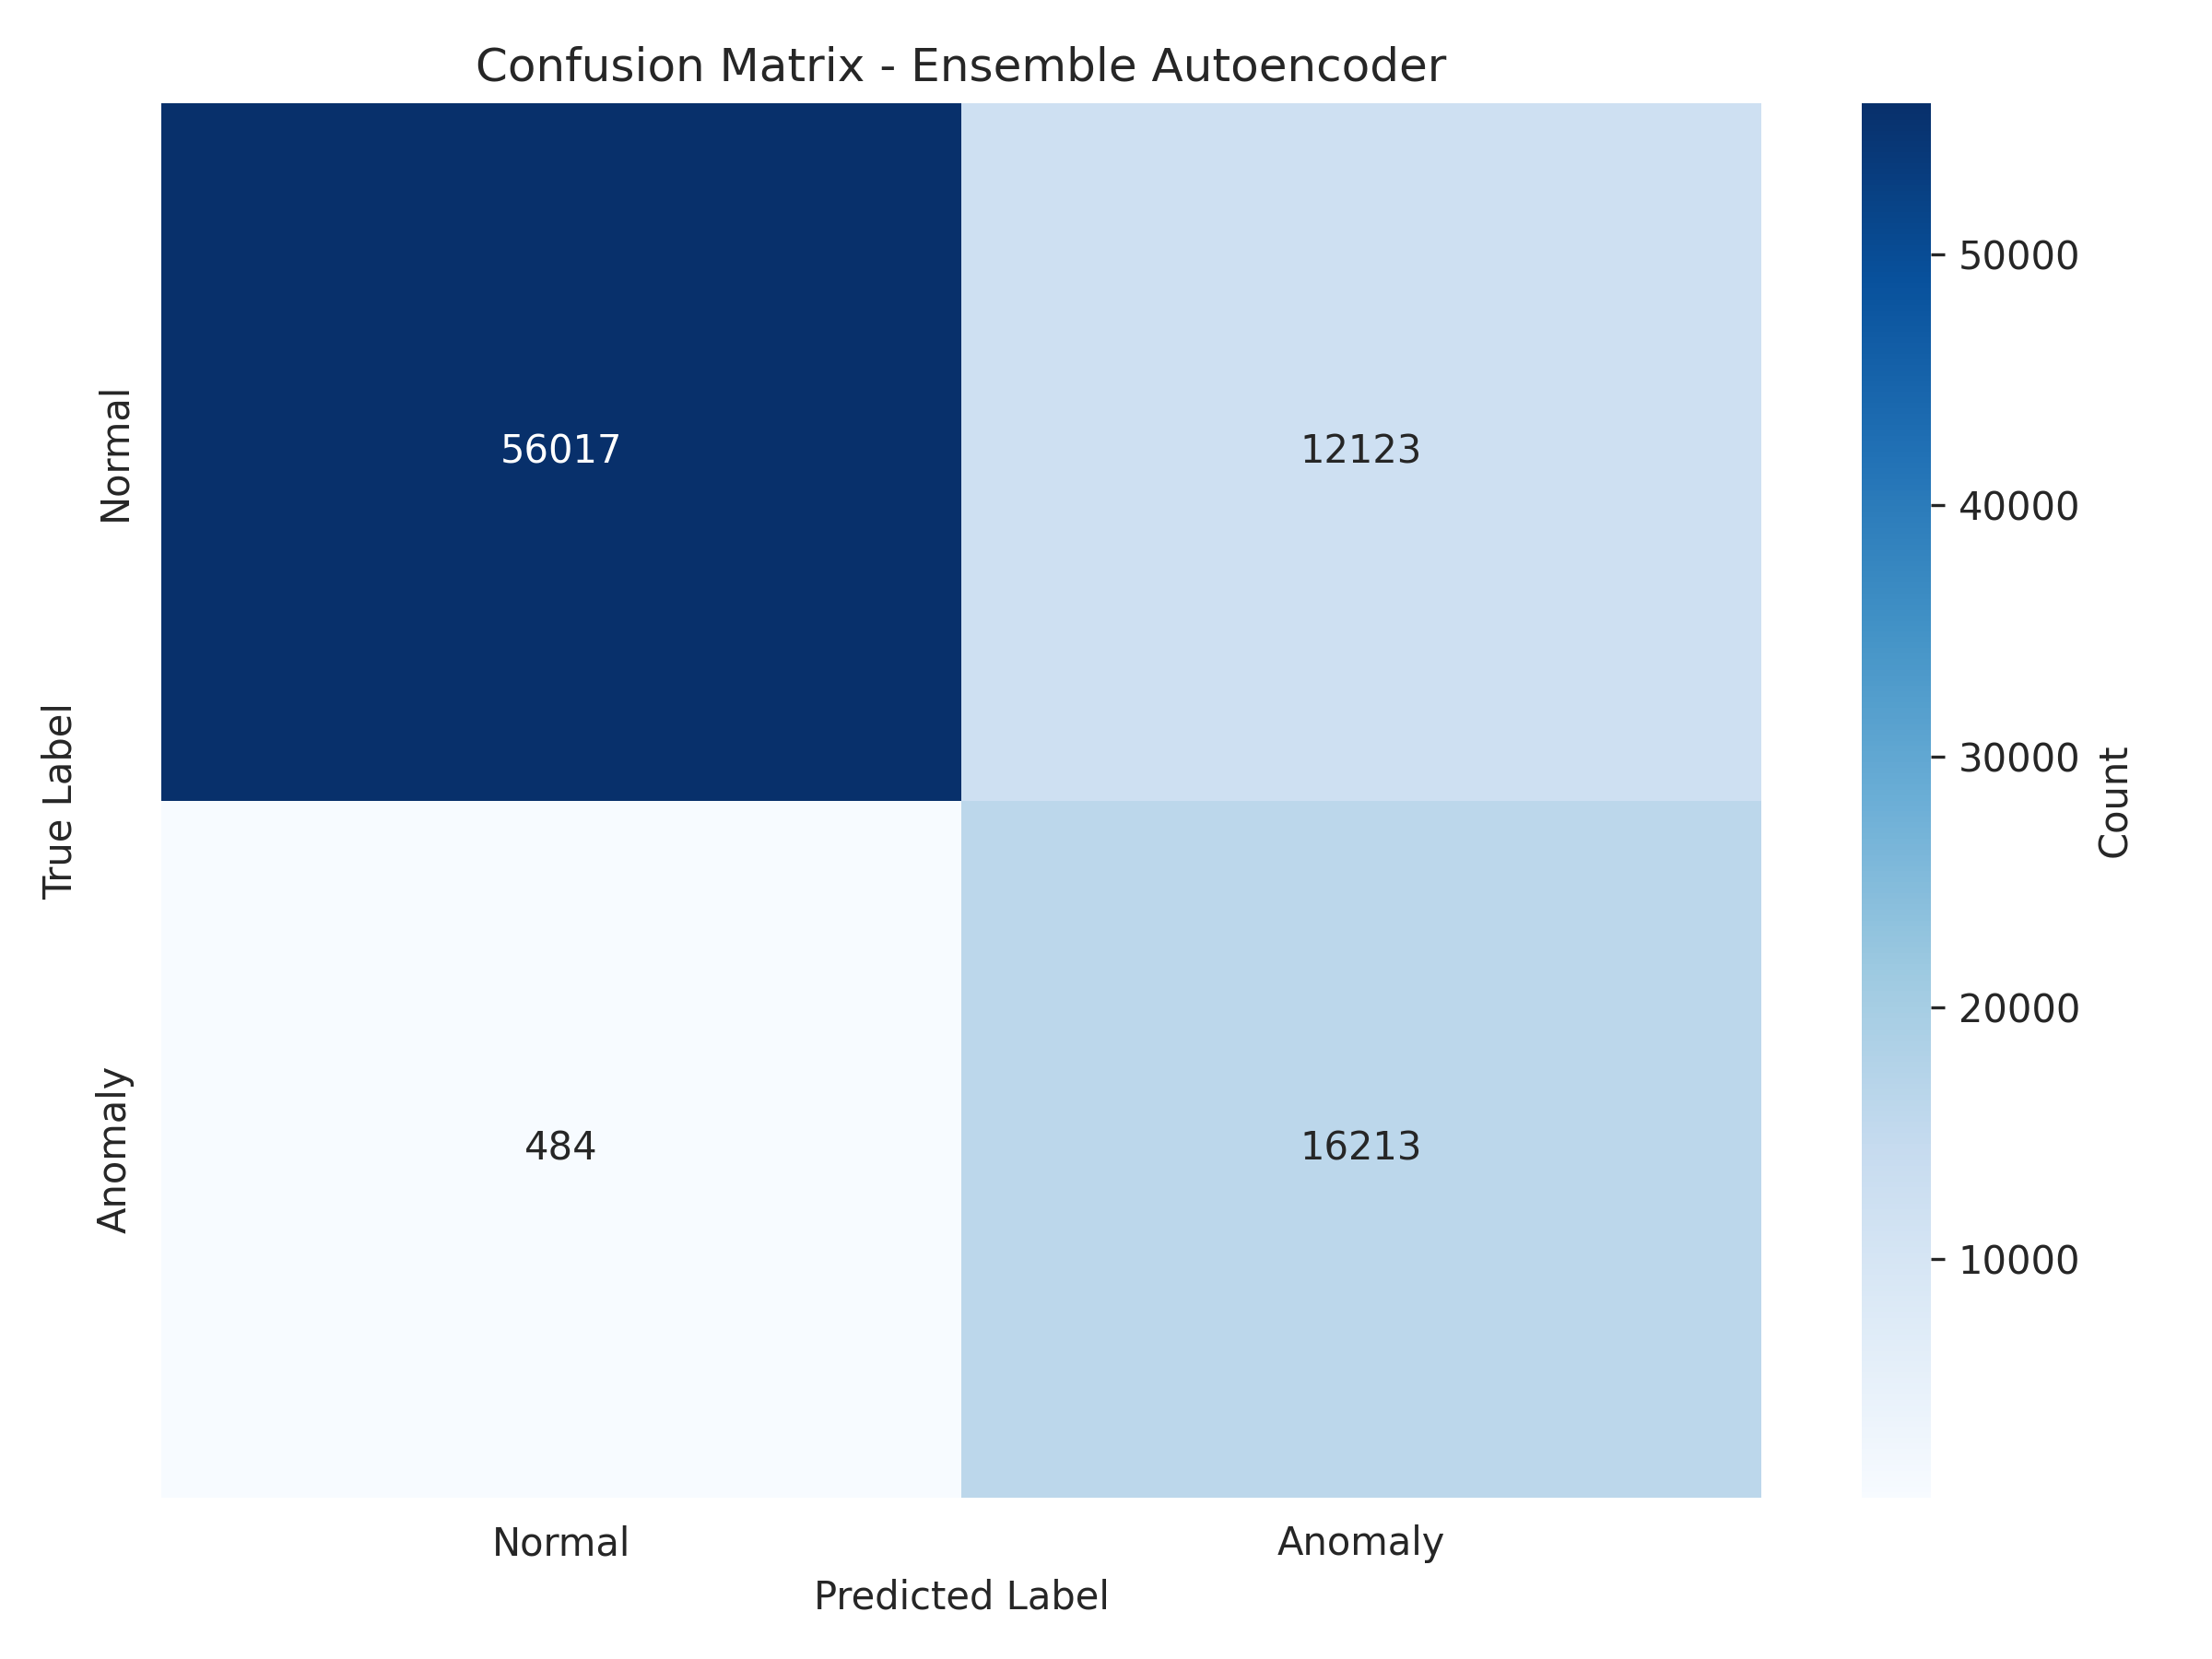
\includegraphics[width=0.46\columnwidth]{../evaluation_results/ensemble_autoencoder_cm.png}
    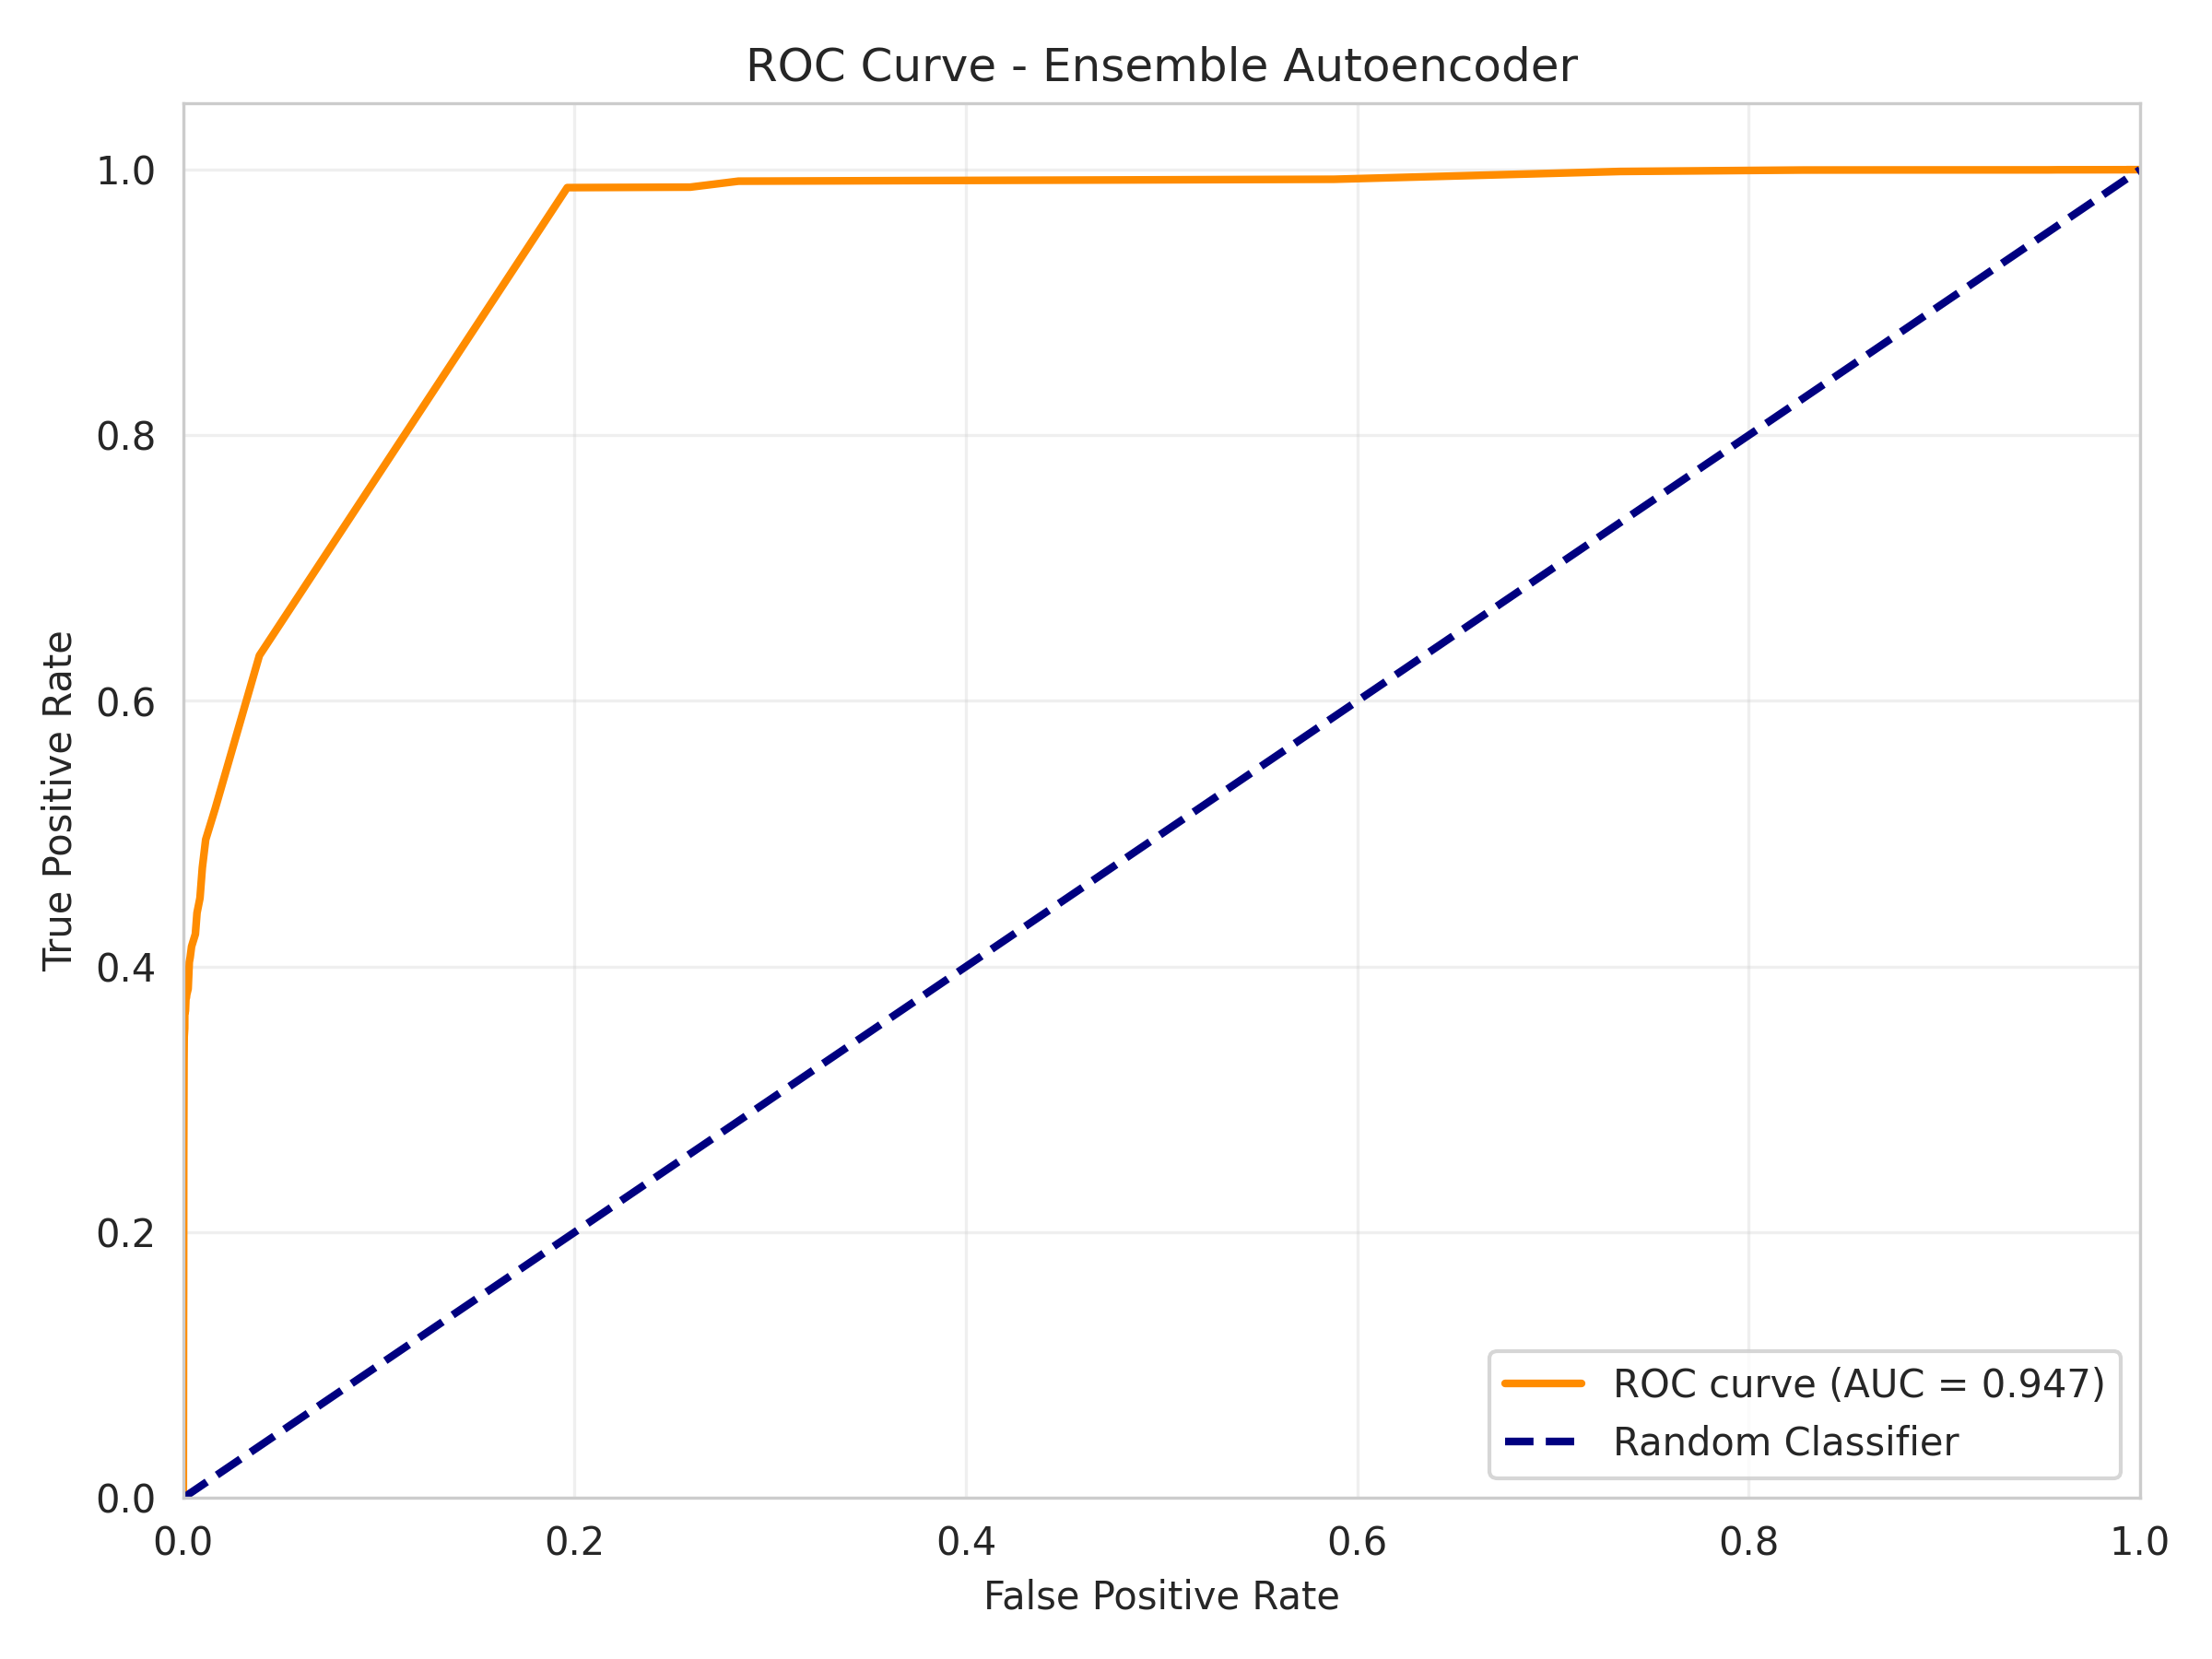
\includegraphics[width=0.46\columnwidth]{../evaluation_results/ensemble_autoencoder_roc.png}
    \caption{Left: Ensemble Autoencoder Confusion Matrix. Right: Ensemble Autoencoder ROC Curve (AUC = 0.947).}
    \label{fig:ensemble_diagnostic}
\end{figure}

The diagnostic outputs for the Ensemble Autoencoder (Figure~\ref{fig:ensemble_diagnostic}) verify its robustness: the ROC curve displays a steep climb, and the confusion matrix shows that out of 16,697 actual anomalies, only 484 are missed (false negatives).

\subsection{Analysis of Overfitting and Underfitting}
A central challenge in unsupervised anomaly detection is balancing model complexity to prevent both underfitting and overfitting:
\begin{itemize}
    \item \textbf{Underfitting in Classical Models:} Local Outlier Factor (LOF) suffers from architectural underfitting if trained with noise. Isolation Forest and OC-SVM baseline models also underfit, failing to capture the complex, multi-vector nature of modern network attacks. In OC-SVM, underfitting occurs when the RBF bandwidth parameter $\gamma$ is too small, making the boundary overly inclusive.
    \item \textbf{Overfitting in Classical Models:} One-Class SVM overfits if the $\gamma$ parameter is too large. This forces the decision boundary to wrap tightly around individual training data points, resulting in high false positive rates during validation. For Isolation Forest, overfitting is primarily controlled by the contamination rate: set too high, normal traffic patterns are incorrectly isolated as anomalies.
    \item \textbf{Deep Learning Models:} The Autoencoders avoid overfitting (i.e., learning the identity mapping) through their contracting bottleneck architecture ($70 \to 32 \to 16 \to 8$). This regularizes the network, forcing it to learn a low-dimensional manifold of normal traffic. Underfitting would occur if the bottleneck were too narrow (e.g., 2 units), preventing the model from reconstructing normal variations. Overfitting is monitored via validation MSE curves (Figure~\ref{fig:loss_comparison}); the training curves demonstrate smooth convergence without validation divergence.
\end{itemize}

% =============================================================


